\chapter{Experimental results}
\indent
	Results of different batch sizes, learning rates, and optimizers are listed in this chapter.
	Experiments of this chapter are done with common setup below: 
	\begin{itemize}
		\item Seed: 42.
		\item Number of epochs: 500.
	\end{itemize} 

\section{Best testing accuracy}
\subsection{EEGNet}
	Best testing accuracy of EEGNet is found with this setup: 
	\begin{itemize}
		\item Optimizer: Adam.
		\item Learning rate: $5 \times 10^{-3}$.
		\item Batch size: 128.
		\item Dropout: 50\%.
	\end{itemize} 
	From Table \ref{eegnet-best-acc-table} and Figure \ref{eegnet-best-acc}, 
	we can see that training and testing accuracy with \code{ReLU} and \code{LeakyReLU} are similar, 
	but accuracy with \code{ELU} is not good enough.

	\begin{table}[htbp]
		\centering
		\begin{tabular}{l|ccc}
			\hline
			\diagbox{Accurcy}{Activation} & ReLU & LeakyReLU & ELU \\ 
			\hline
			\textbf{Testing} & 97.04\% & \textcolor{blue}{\textbf{97.41\%}} & 95.93\% \\ 
			\textbf{Training} & \textcolor{blue}{\textbf{88.52\%}} & 87.87\% & 83.52\% \\ 
			\hline
		\end{tabular}
		\caption{Details of EEGNet best-accuracy setup \\ with different activation functions (\textcolor{blue}{\textbf{Blue}} is the best of each row).}
		\label{eegnet-best-acc-table}
	\end{table}

	\begin{figure}[H]
		\centering
		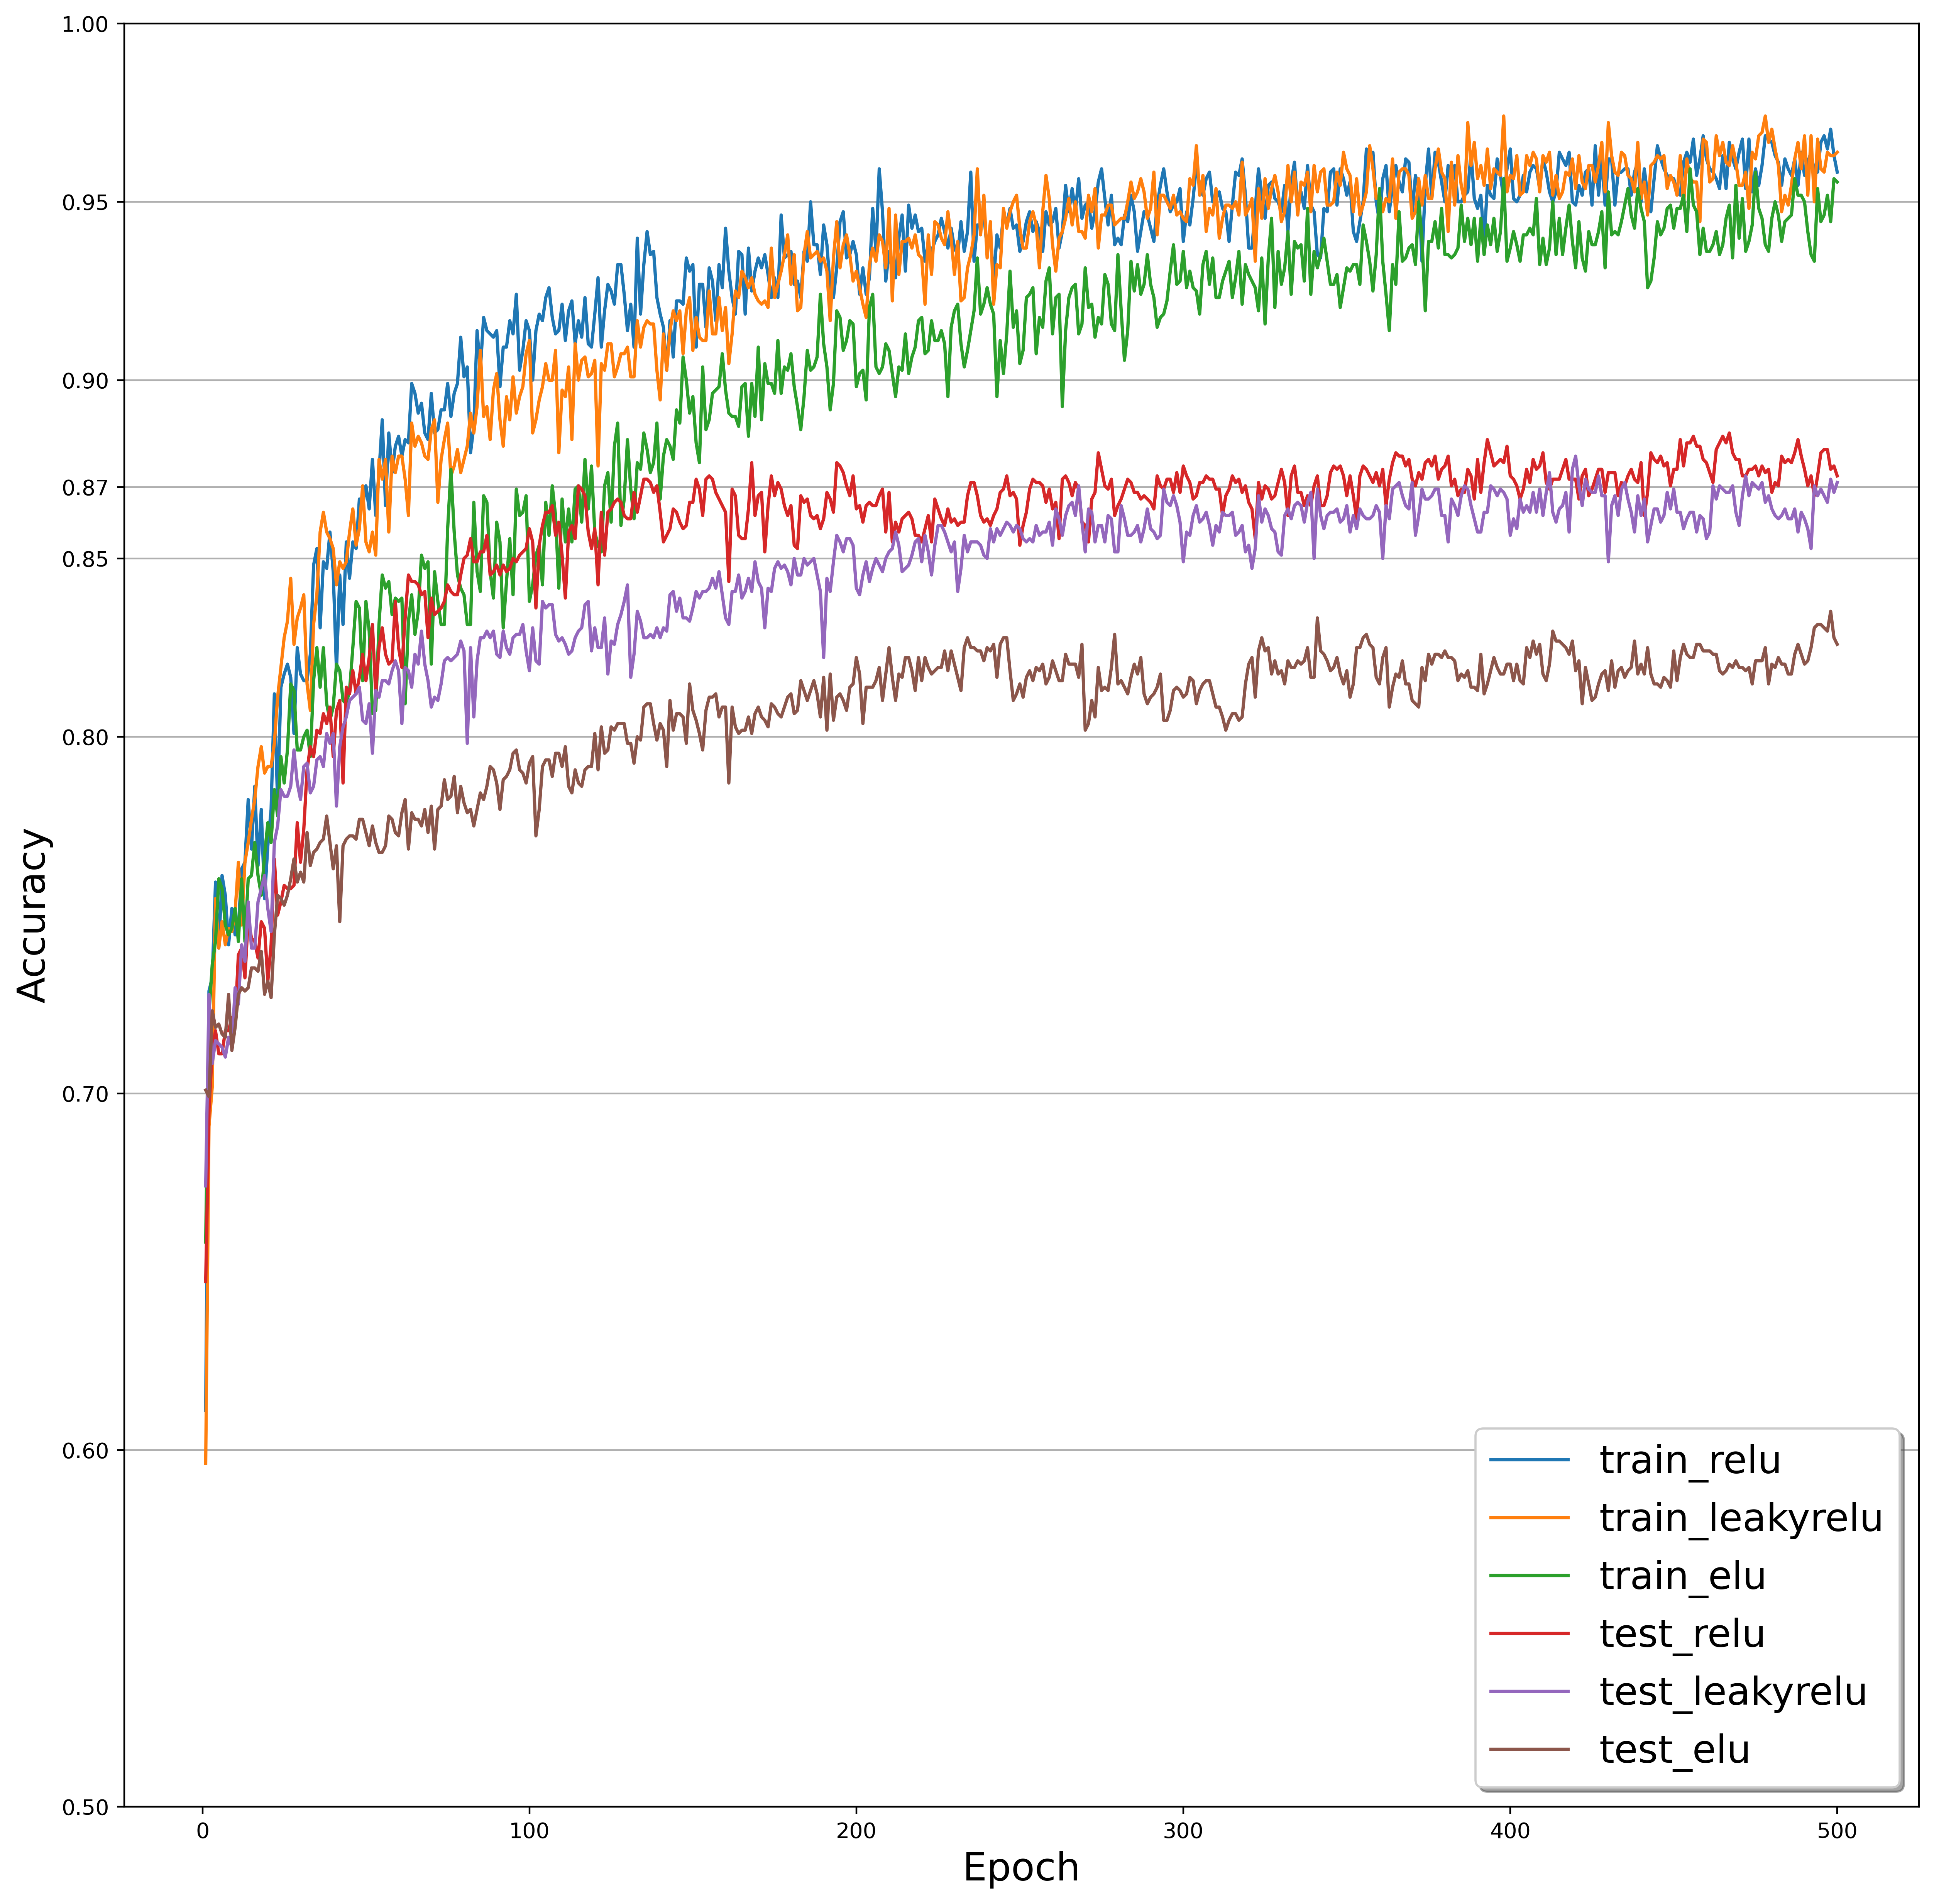
\includegraphics[width=0.45\textwidth]{img/eegnet_adam_128_0.005_0.5_acc.png}
		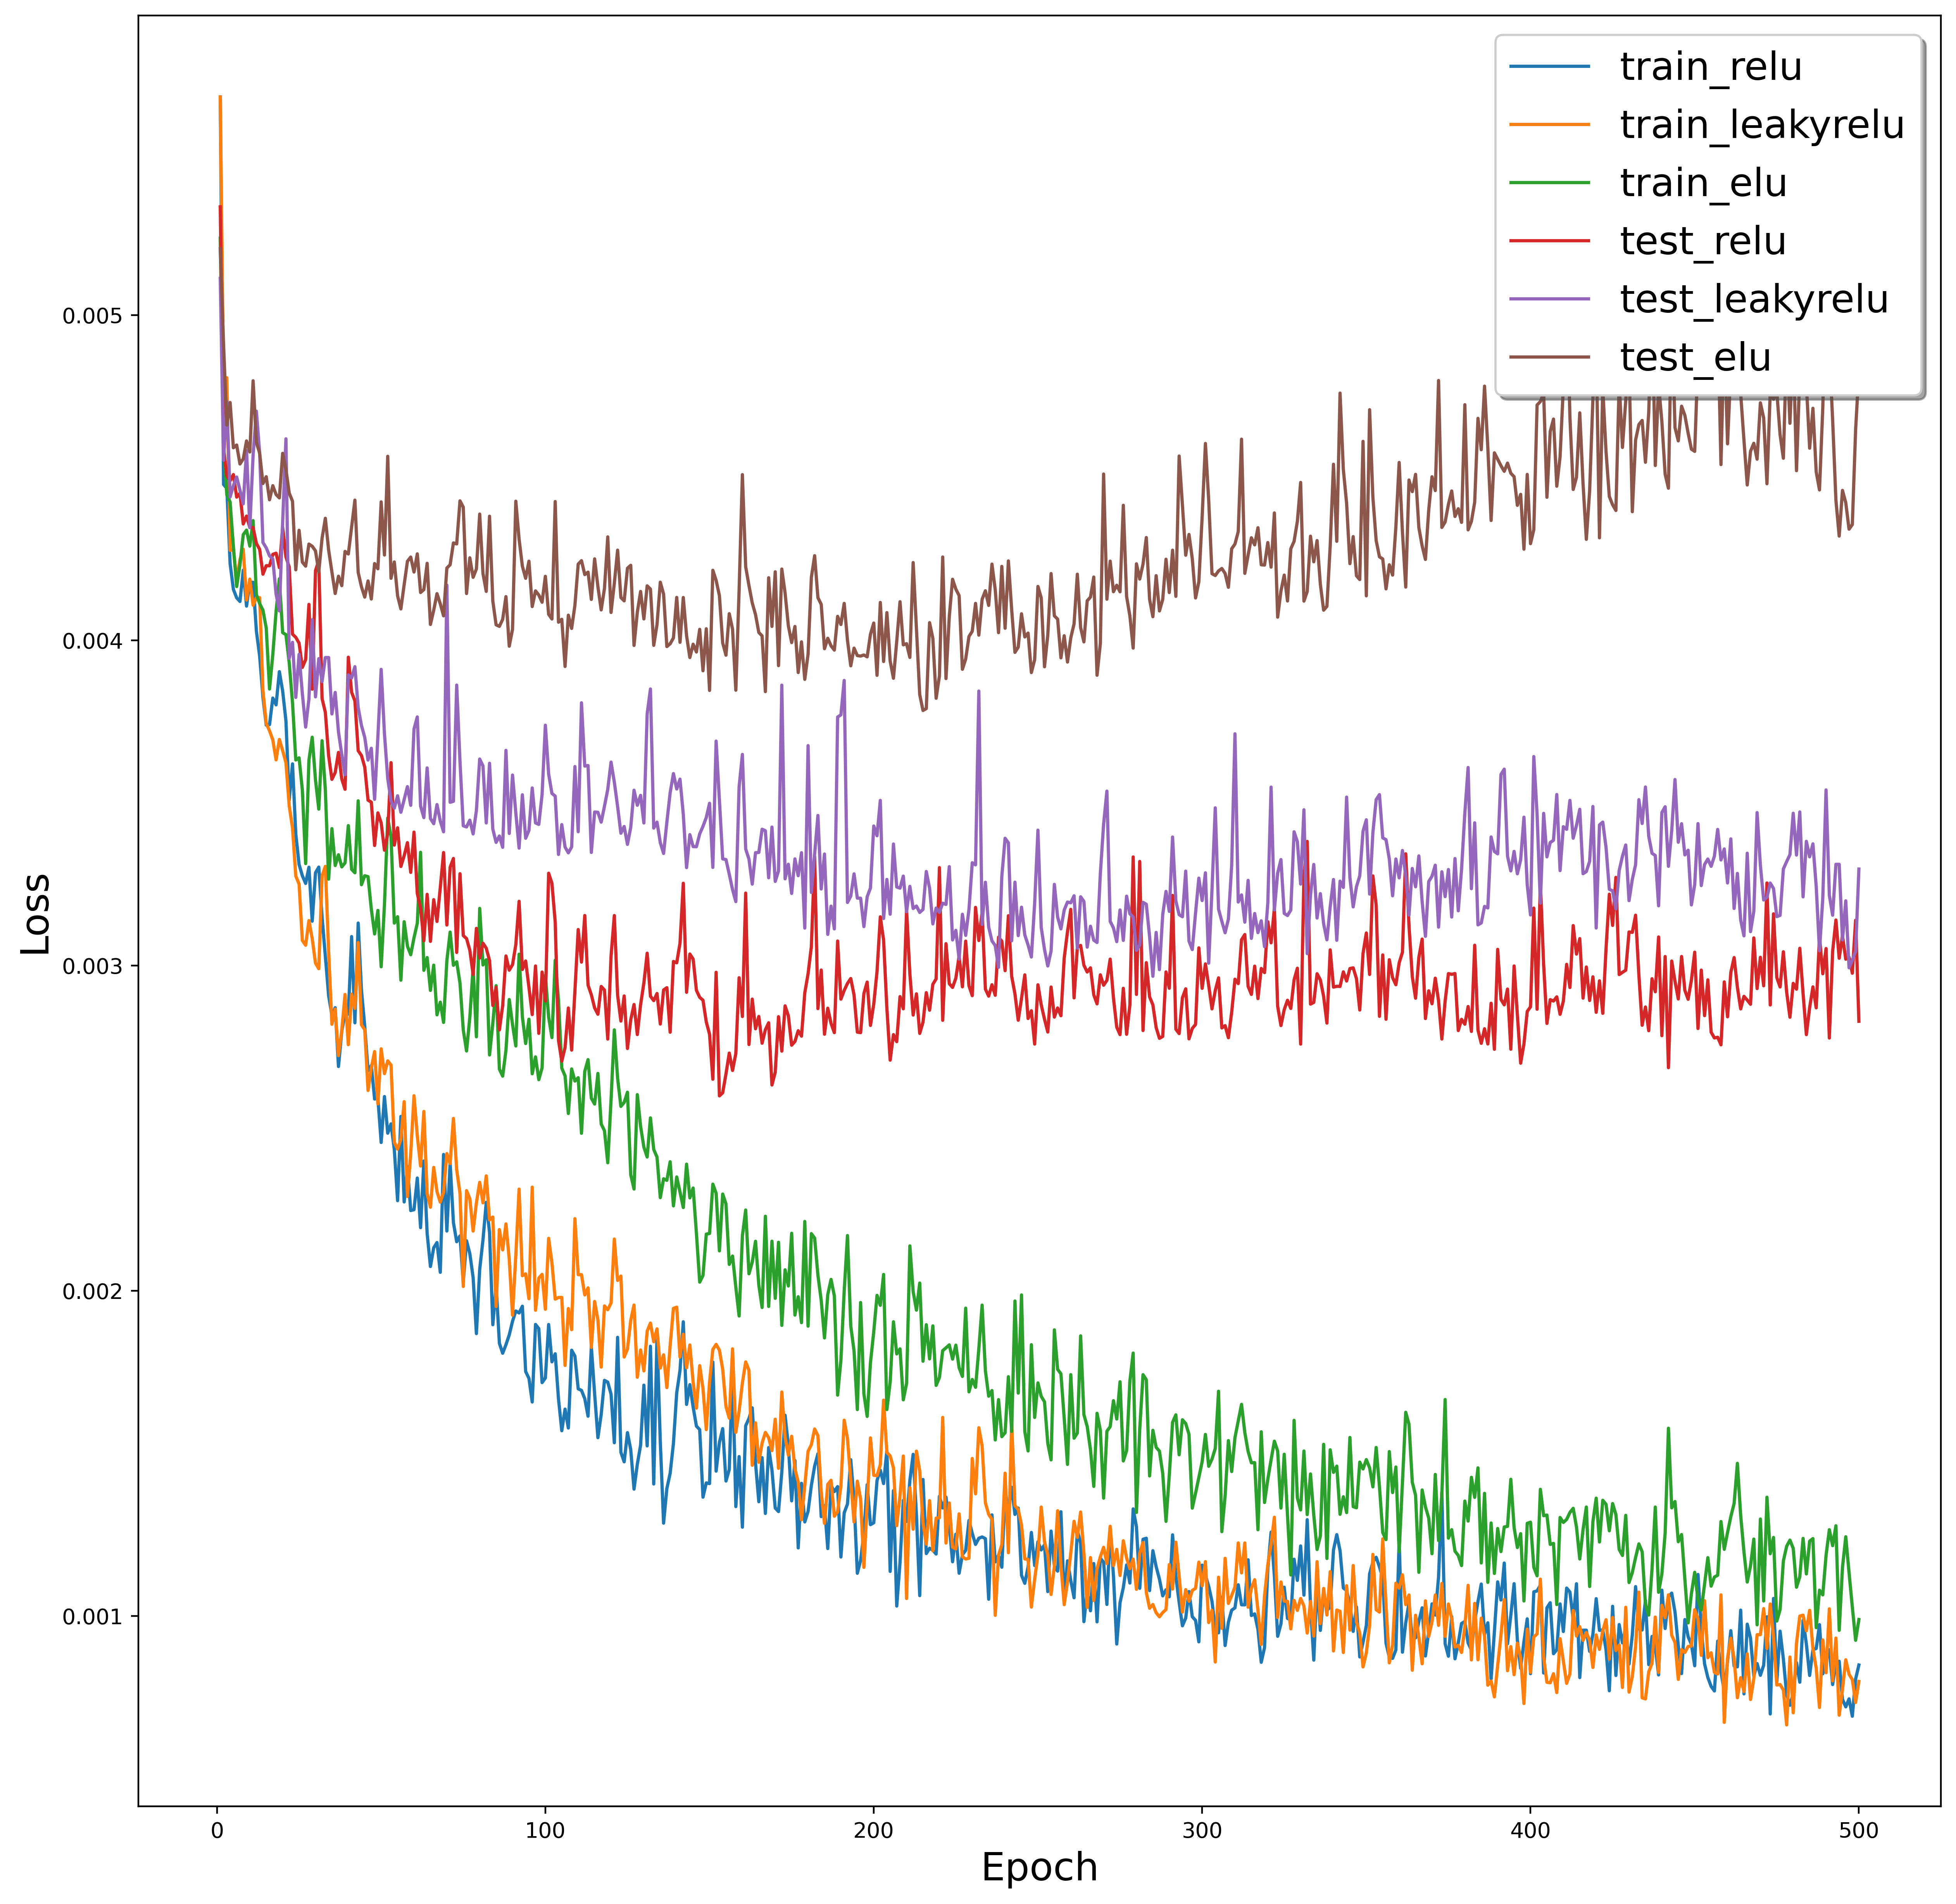
\includegraphics[width=0.45\textwidth]{img/eegnet_adam_128_0.005_0.5_loss.png}
		\caption{Best accuracy of EEGNet and its loss.}
		\label{eegnet-best-acc}
	\end{figure}

	% \begin{figure}[H]
	% 	\centering
	% 	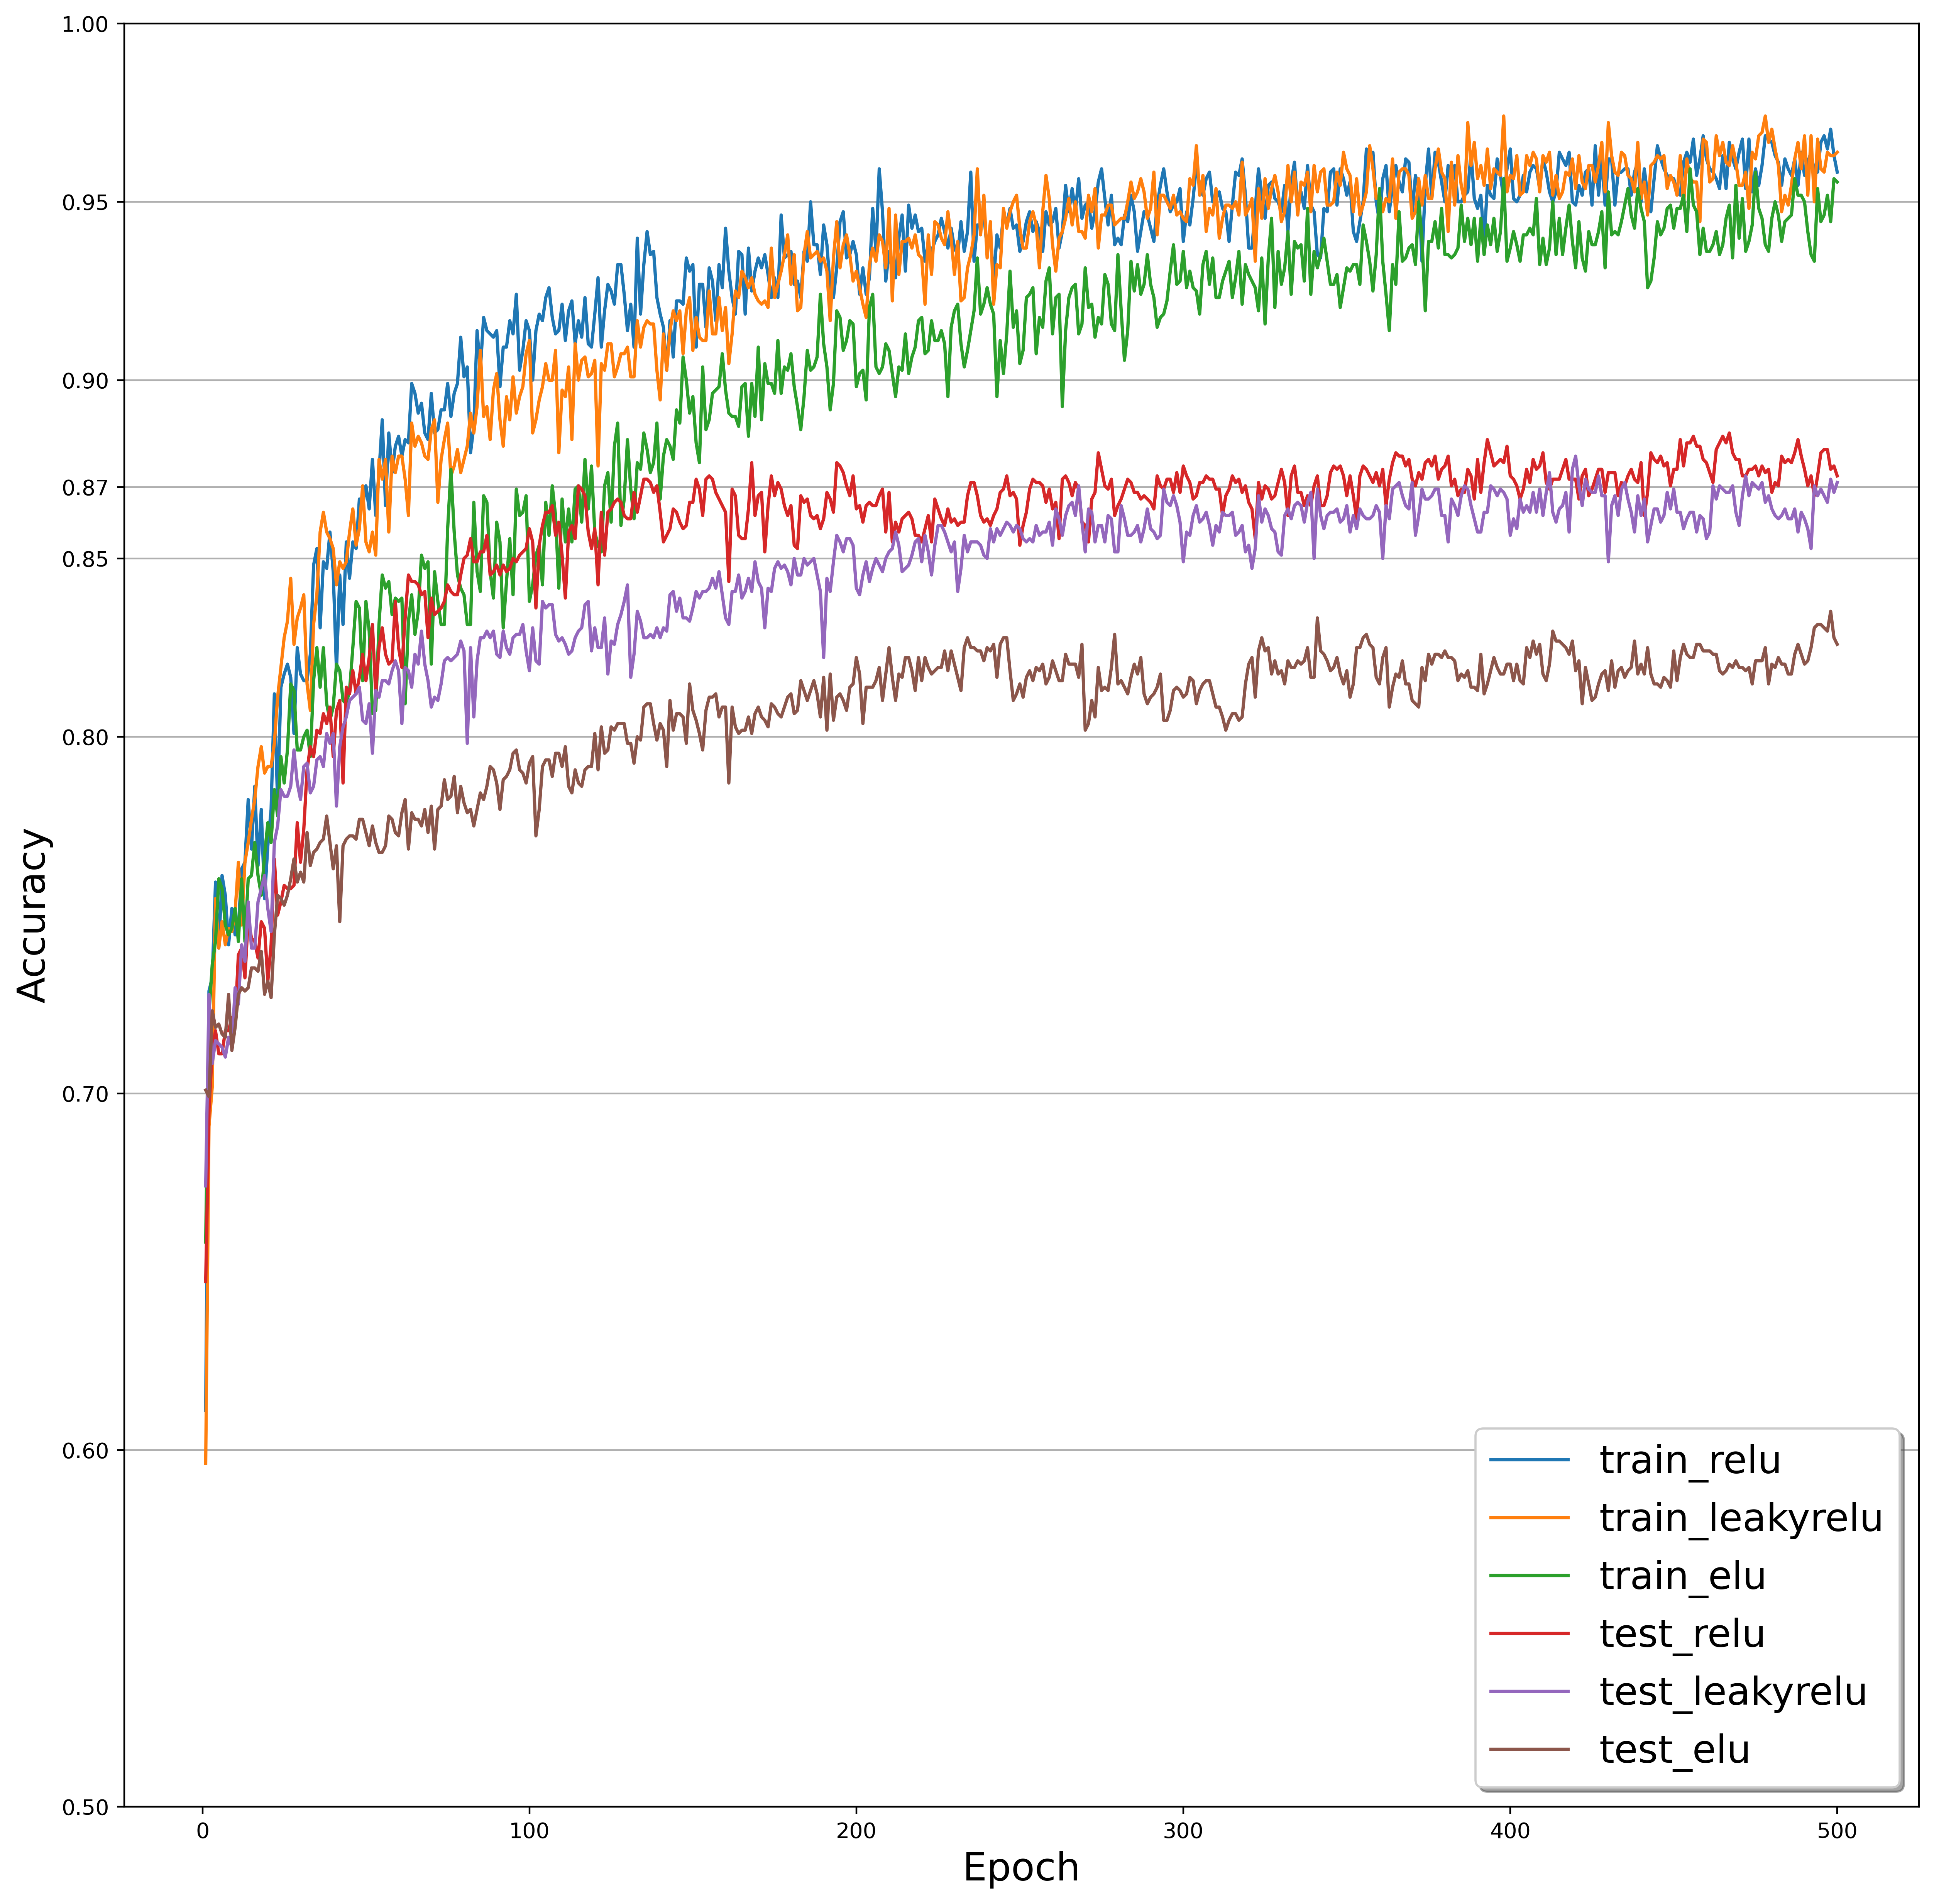
\includegraphics[scale=0.25]{img/eegnet_adam_128_0.005_0.5_acc.png}
	% 	\caption{Best accuracy of EEGNet.}
	% 	\label{eegnet-best-acc-fig}
	% \end{figure}

	% \begin{figure}[H]
	% 	\centering
	% 	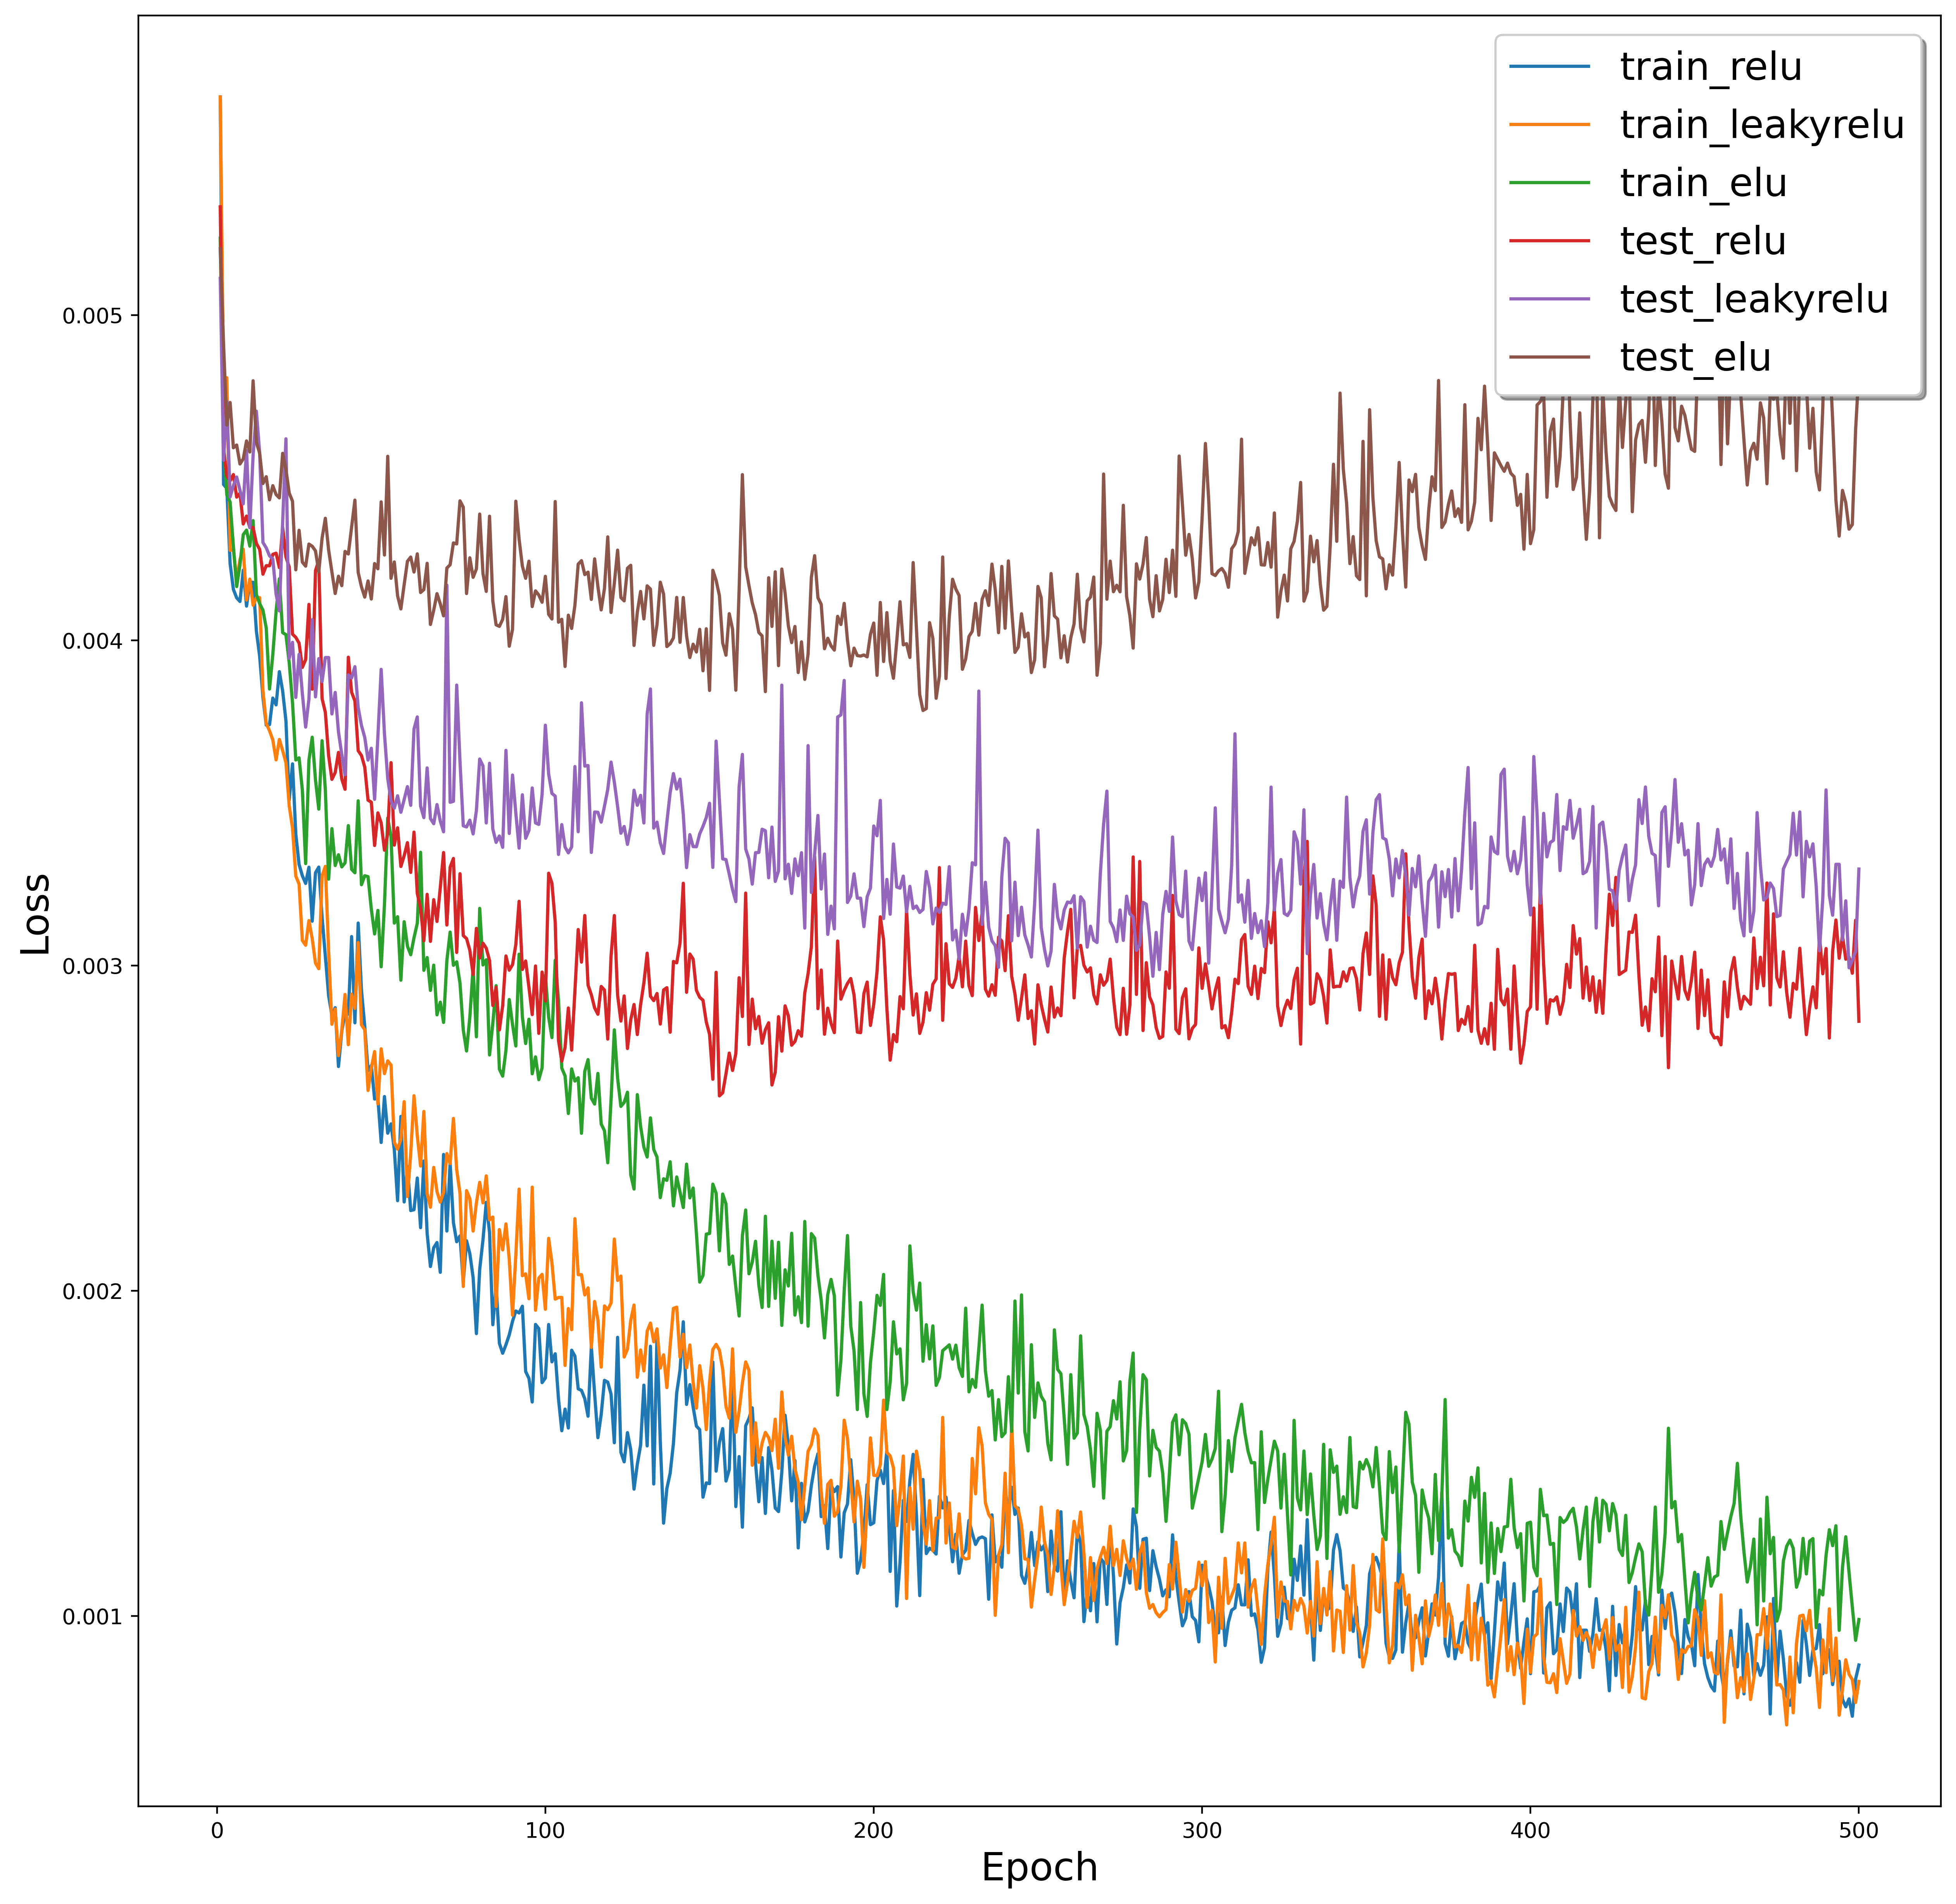
\includegraphics[scale=0.25]{img/eegnet_adam_128_0.005_0.5_loss.png}
	% 	\caption{Loss of best-accuracy EEGNet.}
	% 	\label{eegnet-best-acc-loss}
	% \end{figure}
\pagebreak
\subsection{DeepConvNet}
	Best testing accuracy of DeepConvNet is found with this setup: 
	\begin{itemize}
		\item Optimizer: Adam.
		\item Learning rate: $5 \times 10^{-4}$.
		\item Batch size: 64.
		\item Dropout: 50\%.
	\end{itemize} 
	From Table \ref{deepconvnet-best-acc-table} and Figure \ref{deepconvnet-best-acc}, 
	we can see that training and testing accuracy with each of three activation functions are similar.

	\begin{table}[htbp]
		\centering
		\begin{tabular}{l|ccc}
			\hline
			\diagbox{Accurcy}{Activation} & ReLU & LeakyReLU & ELU \\ 
			\hline
			\textbf{Training} & 95.28\% & 95.65\% & \textcolor{blue}{\textbf{97.87\%}} \\ 
			\textbf{Testing} & \textcolor{blue}{\textbf{82.78\%}} & 82.50\% & 81.02\% \\ 
			\hline
		\end{tabular}
		\caption{Details of DeepConvNet best-accuracy setup \\ with different activation functions (\textcolor{blue}{\textbf{Blue}} is the best of each row).}
		\label{deepconvnet-best-acc-table}
	\end{table}

	\begin{figure}[H]
		\centering
		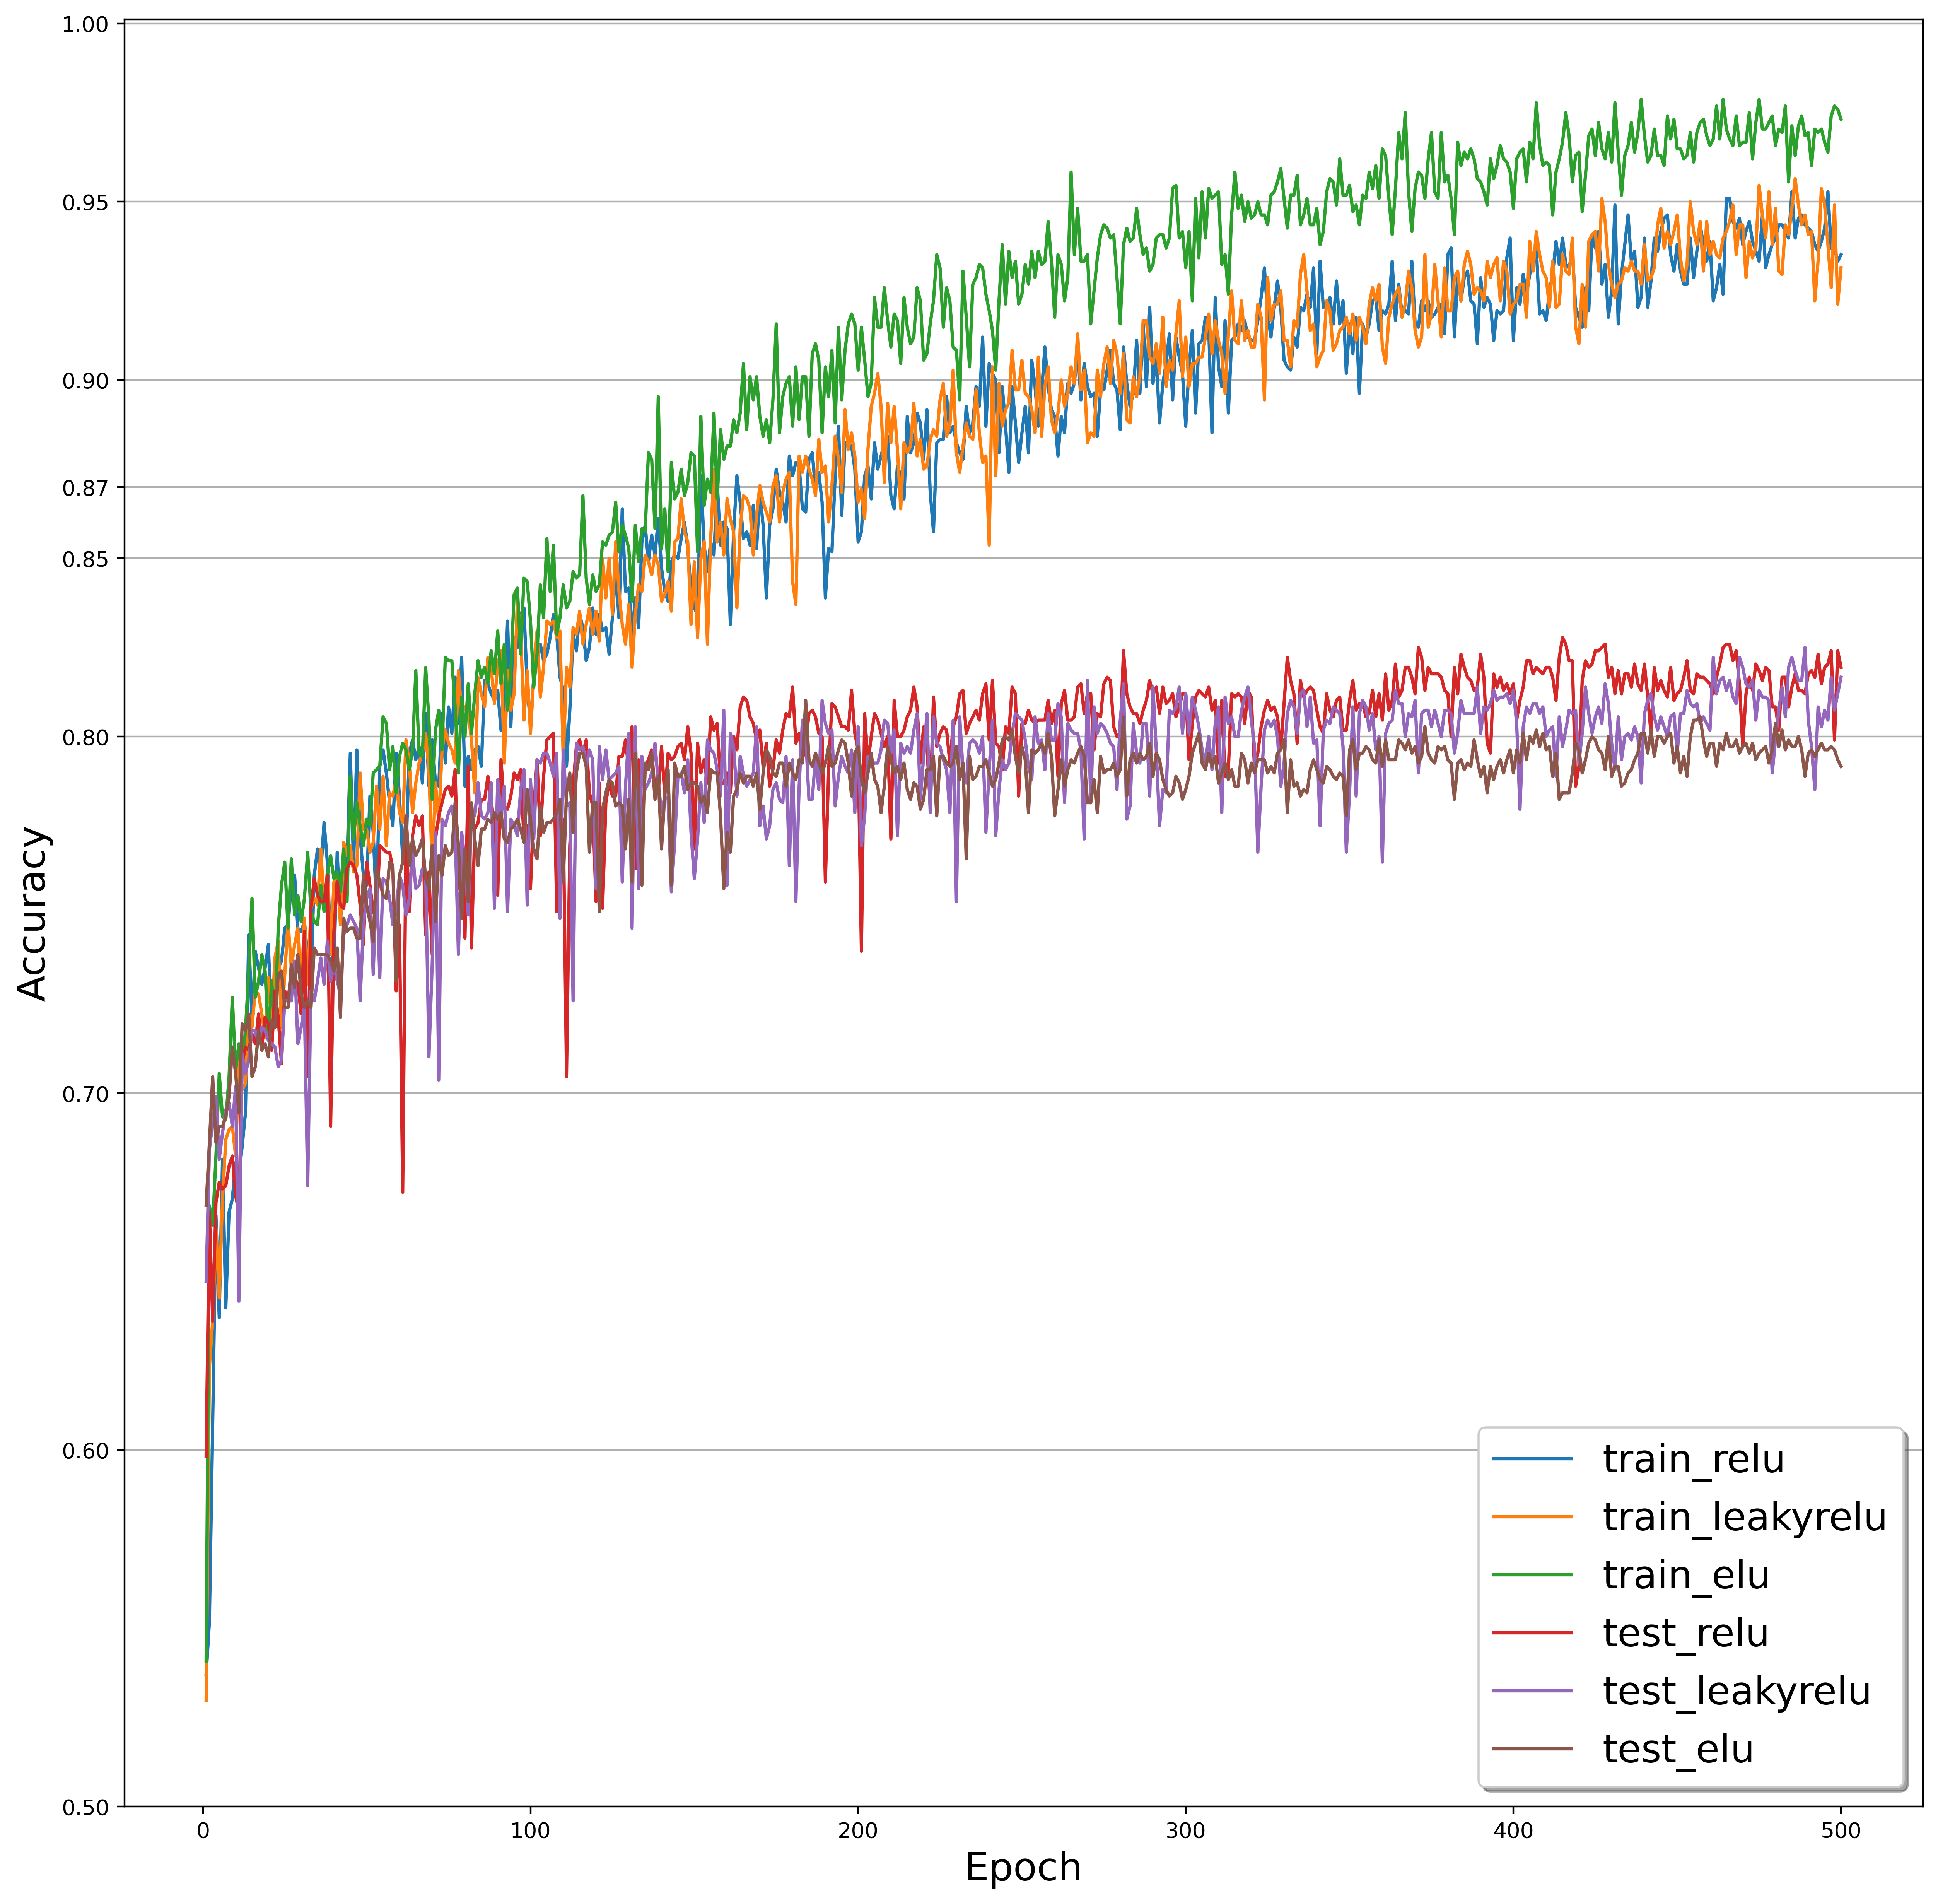
\includegraphics[width=0.45\textwidth]{img/deepconvnet_adam_64_0.0005_0.5_acc.png}
		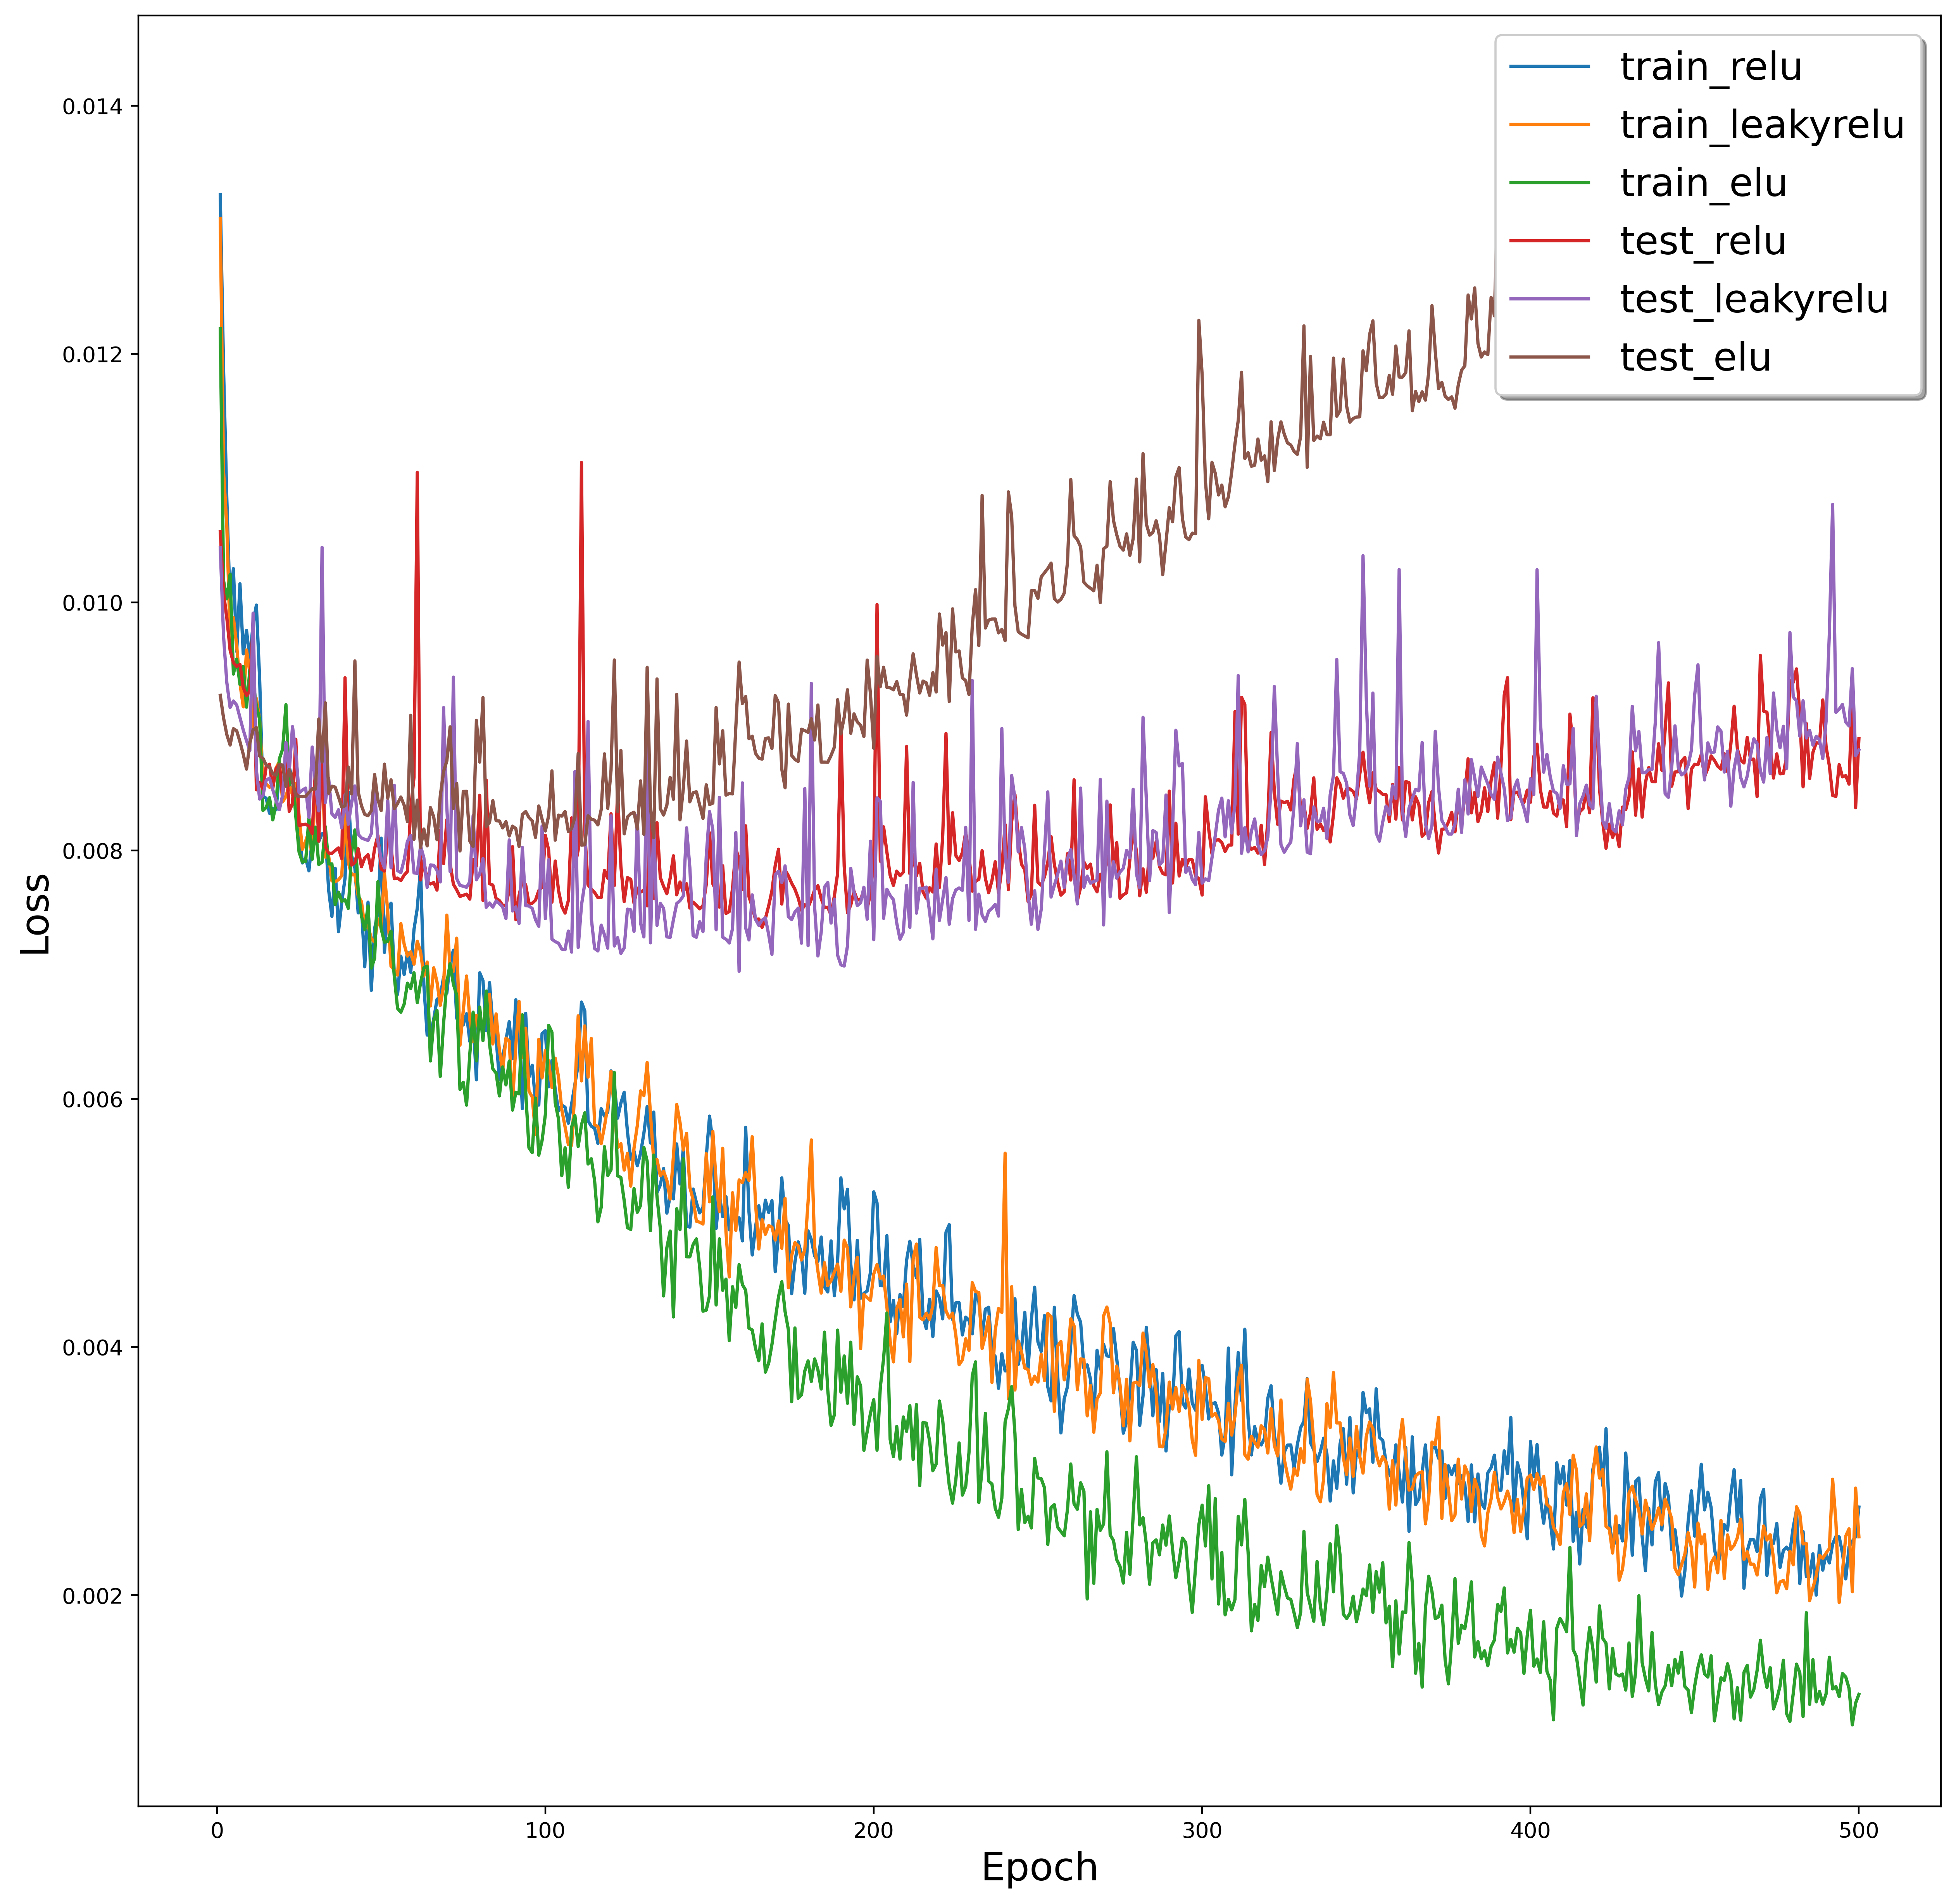
\includegraphics[width=0.45\textwidth]{img/deepconvnet_adam_64_0.0005_0.5_loss.png}
		\caption{Best accuracy of DeepConvNet and its loss.}
		\label{deepconvnet-best-acc}
	\end{figure}

	% \begin{figure}[H]
	% 	\centering
	% 	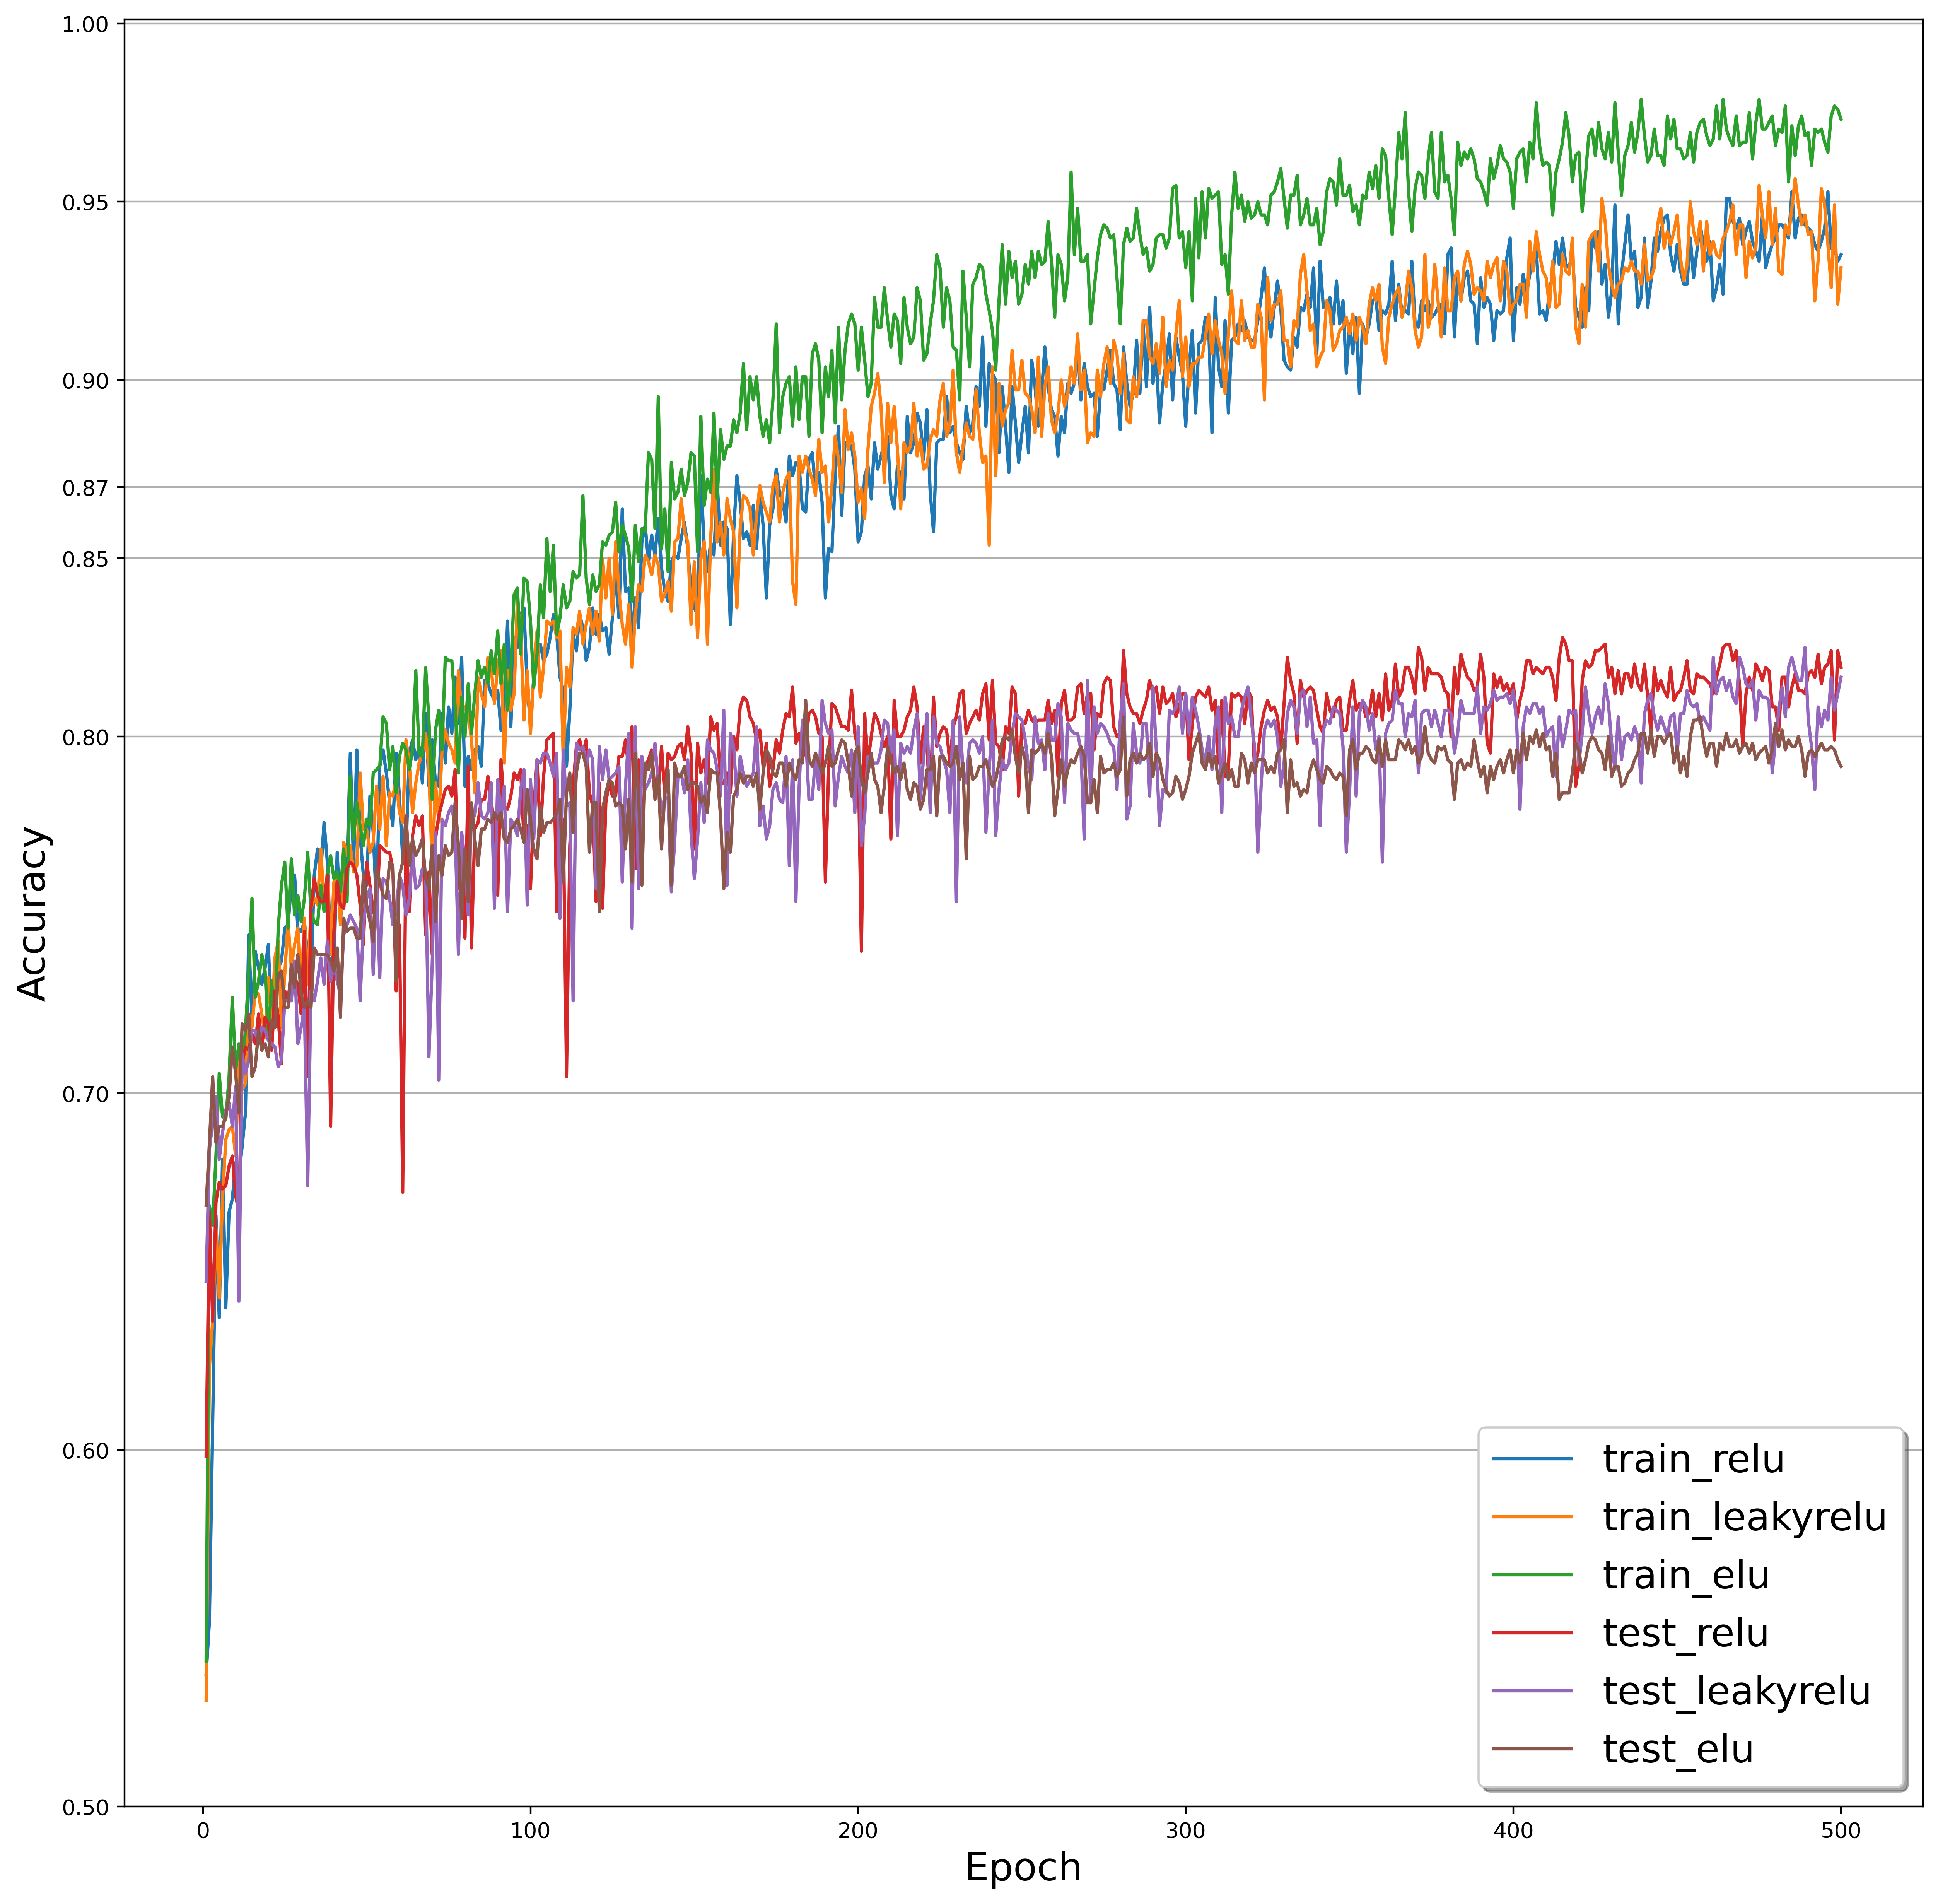
\includegraphics[scale=0.25]{img/deepconvnet_adam_64_0.0005_0.5_acc.png}
	% 	\caption{Best accuracy of DeepConvNet.}
	% 	\label{deepconvnet-best-acc-fig}
	% \end{figure}

	% \begin{figure}[H]
	% 	\centering
	% 	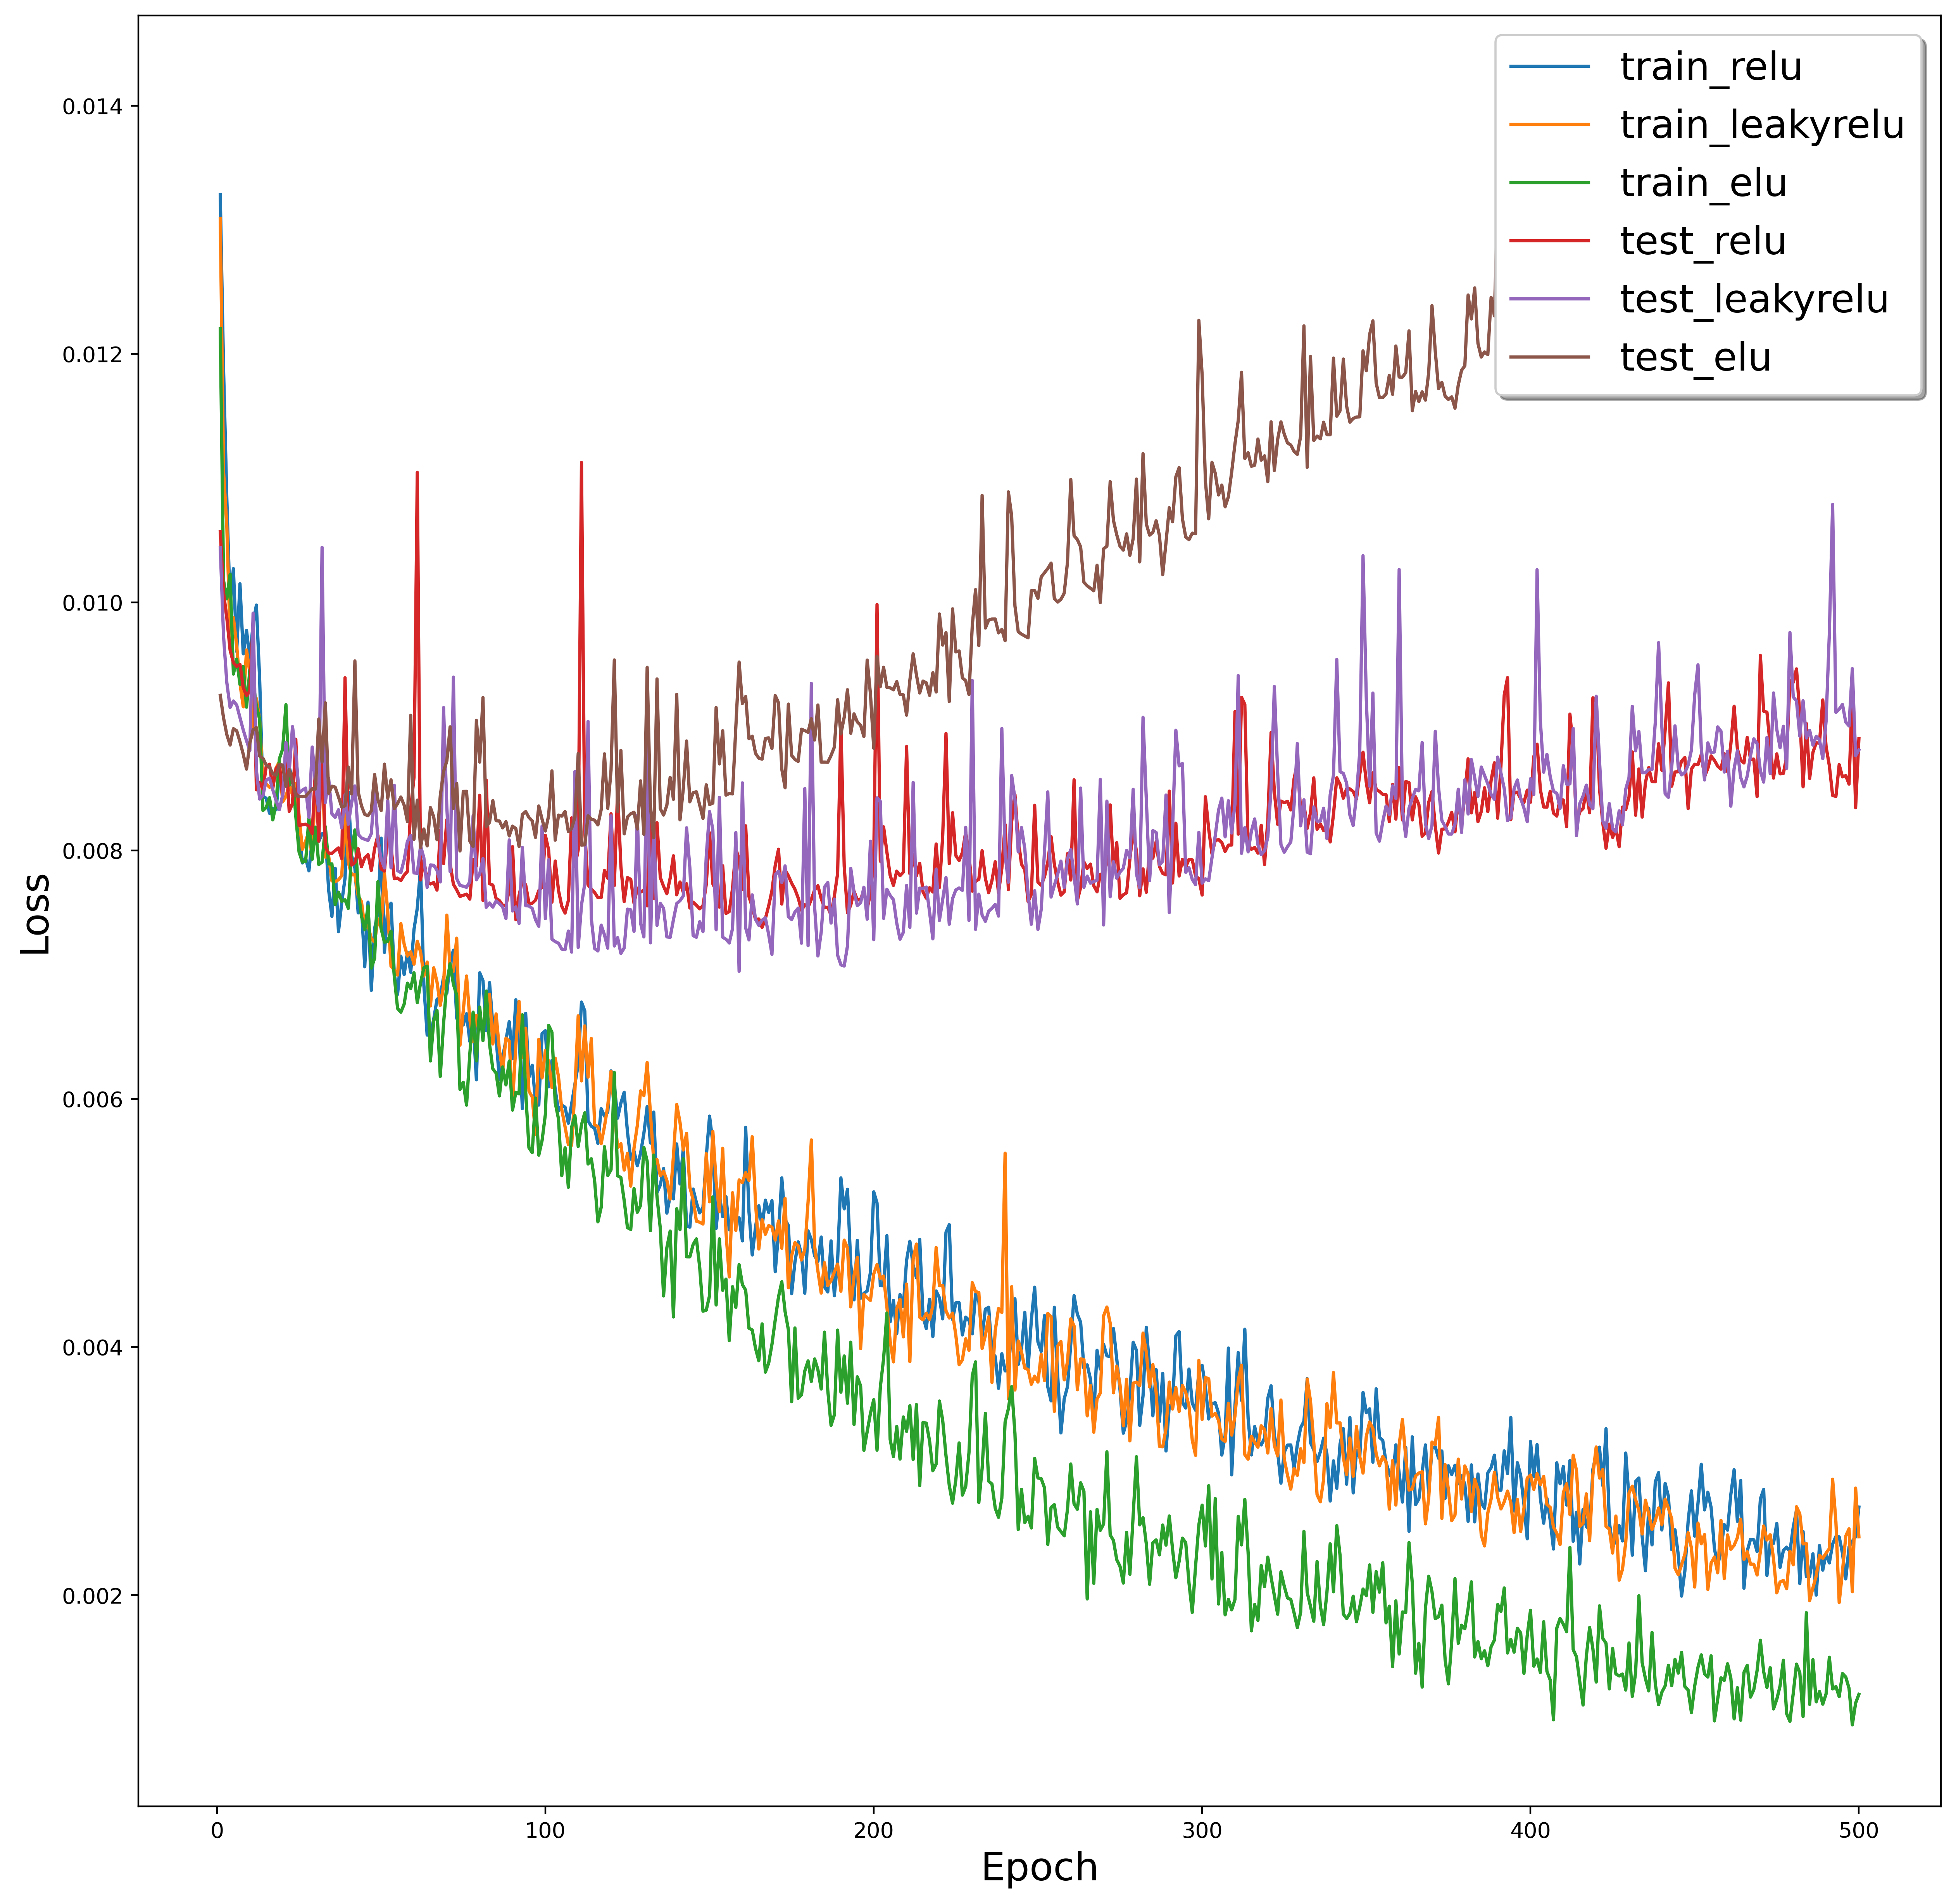
\includegraphics[scale=0.25]{img/deepconvnet_adam_64_0.0005_0.5_loss.png}
	% 	\caption{Loss of best-accuracy DeepConvNet.}
	% 	\label{deepconvnet-best-acc-loss}
	% \end{figure}

\pagebreak
\section{Ablation study}
\subsection{EEGNet}
	From Table \ref{comp-eegnet}, we can see that, in generally, 
	\begin{itemize}
		\item \code{ReLU} and \code{LeakyReLU} do better, and \code{ELU} is always worst. 
		\item Batch size 128 and learning rate $5 \times 10^{-3}$ are best, larger or smaller is worse.
		\item Adam is better than SGD with other setup fixed.
		\item Lower dropout ($25\%$) got higher training accuracy, but a little bit lower for testing. Larger dropout (75\%) is worse on both sets.
	\end{itemize}
	Details are in Chapter \ref{results-eegnet}.

	\begin{table}[htbp]
		\centering
		\resizebox{0.7\linewidth}{!}{
			\begin{tabular}{l|ccc}
				\hline
				\diagbox{Accurcy}{Activation} & ReLU & LeakyReLU & ELU \\ 
				\hline
				\rowcolor{lightgray}
				\textbf{Best} & & & \\
				\rowcolor{lightgray}
				Training & 97.04\% & \textcolor{blue}{\textbf{97.41\%}} & 95.93\% \\
				\rowcolor{lightgray}
				Testing & \textcolor{blue}{\textbf{88.52\%}}\textsuperscript{\textdagger} & 87.87\% & 83.52\% \\ 
				\Xhline{3\arrayrulewidth}
				\textbf{Smaller batch size (64)} & & & \\
				Training & 97.41\% & \textcolor{blue}{\textbf{97.50\%}} & 95.65\% \\ 
				Testing & \textcolor{blue}{\textbf{87.78\%}} & 86.57\% & 82.50\% \\ 
				\Xhline{3\arrayrulewidth}
				\textbf{Larger batch size (256)} & & & \\
				Training & \textcolor{blue}{\textbf{97.04\%}} & 96.39\% & 95.83\% \\ 
				Testing & \textcolor{blue}{\textbf{87.59\%}} & 86.85\% & 83.98\%\textsuperscript{\textdagger} \\ 
				\Xhline{3\arrayrulewidth}
				\textbf{Smaller learning rate ($1 \times 10^{-3}$) } & & & \\
				Training & 94.91\% & \textcolor{blue}{\textbf{96.20\%}} & 93.98\% \\ 
				Testing & 86.20\% & \textcolor{blue}{\textbf{88.33\%}}\textsuperscript{\textdagger} & 83.89\% \\ 
				\Xhline{3\arrayrulewidth}
				\textbf{Larger learning rate ($1 \times 10^{-2}$)} & & & \\ 
				Training & \textcolor{blue}{\textbf{97.31\%}} & 97.04\% & 95.00\% \\ 
				Testing & \textcolor{blue}{\textbf{86.39\%}} & 85.28\% & 83.15\% \\ 
				\Xhline{3\arrayrulewidth}
				\textbf{Different optimizer (SGD)} & & & \\
				Training & \textcolor{blue}{\textbf{93.24\%}} & 93.15\% & 91.57\% \\ 
				Testing & 85.65\% & \textcolor{blue}{\textbf{86.30\%}} & 81.20\% \\
				\Xhline{3\arrayrulewidth}
				\textbf{Smaller dropout (25\%)} & & & \\
				Training & \textcolor{blue}{\textbf{99.91\%}}\textsuperscript{\textdagger} & \textcolor{blue}{\textbf{99.91\%}}\textsuperscript{\textdagger} & 99.72\%\textsuperscript{\textdagger} \\ 
				Testing & \textcolor{blue}{\textbf{87.04\%}} & 86.11\% & 82.69\% \\
				\Xhline{3\arrayrulewidth}
				\textbf{Larger dropout (75\%)} & & & \\
				Training & 90.28\% & \textcolor{blue}{\textbf{90.37\%}} & 84.72\% \\ 
				Testing & \textcolor{blue}{\textbf{87.04\%}} & 86.39\% & 82.13\% \\
				\hline
			\end{tabular}}
			\caption{Ablation study of EEGNet. \\ (\textcolor{blue}{\textbf{Blue}} is the best of each row, \textsuperscript{\textdagger} is the best of each activation function).}
			\label{comp-eegnet}
		\end{table}

\subsection{DeepConvNet}
	From Table \ref{comp-deepconvnet}, we can see that, in generally, 
	\begin{itemize}
		\item Accuracy of each activation function is similar.
		\item Batch size 64 and learning rate $5 \times 10^{-4}$ are best, larger or smaller is worse.
		\item Adam is better than SGD with other setup fixed.
		\item Lower dropout ($25\%$) got higher training accuracy, but a little bit lower for testing. Larger dropout (75\%) is worse on both sets.
	\end{itemize}
	Details are in Chapter \ref{results-deepconvnet}.
	
	\begin{table}[htbp]
		\centering
		\resizebox{0.7\linewidth}{!}{
			\begin{tabular}{l|ccc}
				\hline
				\diagbox{Accurcy}{Activation} & ReLU & LeakyReLU & ELU \\ 
				\hline
				\rowcolor{lightgray}
				\textbf{Best} & & & \\
				\rowcolor{lightgray}
				Training & 95.28\% & 95.65\% & \textcolor{blue}{\textbf{97.87\%}} \\ 
				\rowcolor{lightgray}
				Testing & \textcolor{blue}{\textbf{82.78\%}}\textsuperscript{\textdagger} & 82.50\%\textsuperscript{\textdagger} & 81.02\% \\
				\Xhline{3\arrayrulewidth}
				\textbf{Smaller batch size (32)} & & & \\
				Training & 96.02\% & 97.57\% & \textcolor{blue}{\textbf{98.43\%}} \\ 
				Testing & 80.65\% & 80.56\% & \textcolor{blue}{\textbf{81.02\%}} \\ 
				\Xhline{3\arrayrulewidth}
				\textbf{Larger batch size (128)} & & & \\
				Training & 93.43\% & 94.17\% & \textcolor{blue}{\textbf{96.94\%}} \\ 
				Testing & \textcolor{blue}{\textbf{81.76\%}} & 81.67\% & 80.19\% \\ 
				\Xhline{3\arrayrulewidth}
				\textbf{Smaller learning rate ($1 \times 10^{-4}$) } & & & \\
				Training & 86.39\% & 87.13\% & \textcolor{blue}{\textbf{88.70\%}} \\ 
				Testing & 80.19\% & \textcolor{blue}{\textbf{81.11\%}} & 79.17\% \\ 
				\Xhline{3\arrayrulewidth}
				\textbf{Larger learning rate ($1 \times 10^{-3}$)} & & & \\ 
				Training & 97.22\% & 97.78\% & \textcolor{blue}{\textbf{98.89\%}} \\ 
				Testing & 81.57\% & \textcolor{blue}{\textbf{82.04\%}} & 81.39\%\textsuperscript{\textdagger} \\ 
				\Xhline{3\arrayrulewidth}
				\textbf{Different optimizer (SGD)} & & & \\ 
				Training & 81.76\% & 82.69\% & \textcolor{blue}{\textbf{84.26\%}} \\ 
				Testing & 78.24\% & 78.06\% & \textcolor{blue}{\textbf{78.61\%}} \\
				\Xhline{3\arrayrulewidth}
				\textbf{Smaller dropout (25\%)} & & & \\ 
				Training & \textcolor{blue}{\textbf{100.00\%}}\textsuperscript{\textdagger} & \textcolor{blue}{\textbf{100.00\%}}\textsuperscript{\textdagger} & \textcolor{blue}{\textbf{100.00\%}}\textsuperscript{\textdagger} \\ 
				Testing & \textcolor{blue}{\textbf{82.13\%}} & 81.48\% & 80.46\% \\
				\Xhline{3\arrayrulewidth}
				\textbf{Larger dropout (75\%)} & & & \\ 
				Training & 80.09\% & \textcolor{blue}{\textbf{82.13\%}} & 81.20\% \\ 
				Testing & 77.87\% & 78.33\% & \textcolor{blue}{\textbf{78.98\%}} \\
				\hline
			\end{tabular}}
			\caption{Ablation study of DeepConvNet. \\ (\textcolor{blue}{\textbf{Blue}} is the best of each row, \textsuperscript{\textdagger} is the best of each activation function).}
			\label{comp-deepconvnet}
		\end{table}
